
\documentclass[conference]{IEEEtran}
\IEEEoverridecommandlockouts%
\usepackage{cite}
\usepackage{newtxtext,newtxmath}
\usepackage{booktabs}
%\usepackage[a4paper,margin=1in]{geometry}
%\usepackage{parskip}
\usepackage{amsmath}
\usepackage{graphicx}
\usepackage{hyperref}
\hypersetup{colorlinks, citecolor=blue}
\usepackage{tabularx}

\title{KV Cache Optimization in LLMs: A Taxonomy and Decision Framework for Efficient Inference}
\author{
	\IEEEauthorblockN{1\textsuperscript{st} Aayush Chhuka}
	\IEEEauthorblockA{\textit{Department of Computer Science and Engineering} \\
		\textit{National College of Engineering}\\
		Lalitapur, Nepal \\
		aayushchhuka20@gmail.com}
	
	\and
	
	\IEEEauthorblockN{2\textsuperscript{nd} Aditya Brajacharya}
	\IEEEauthorblockA{\textit{Department of Computer Science and Engineering} \\
		\textit{National College of Engineering}\\
		Lalitapur, Nepal \\
		aadityabrjacharya123@gmail.com}
	
	\and
	\IEEEauthorblockN{3\textsuperscript{rd} Sudip Dhungana}
	\IEEEauthorblockA{\textit{Department of Computer Science and Engineering} \\
		\textit{National College of Engineering}\\
		Lalitapur, Nepal \\
		sudipdhungana02@gmail.com}
}
\begin{document}
\maketitle
\section{Introduction}
Recently, Large Language Models (LLMs) have become a core foundation in AI-driven applications due to the sole reason of powerful understanding and generation of natural language. Unlike traditional AI systems, LLMs provide great flexibility and handle wide range of tasks with enhanced adaptability~\cite{shan2025cognitivememoryllms}. To manage active information, LLMs utilize a short-term memory technique known as the context window. Within this window, the model processes previous conversational turns, external documents, and its own prior outputs. To generate logical text, LLMs rely on an autoregressive process which generates tokens one by one based on all previous tokens to understand the broader context of the sequence~\cite{nvidia2025nvfp4}.

A main challenge for LLM deployment is how models manage, access and retain information across interactions. Due to this autoregressive behaviour, the computing cost of a model increases as it recalculates the mathematical relation of previous tokens each and every time a new token is generated~\cite{nvidia2025nvfp4}. This leads to computational overhead within the context window. In some cases input context can be tens and hundreds of times longer than the output it generates~\cite{lu2026mixquant}.

To overcome the limitation of recomputation of past token, the key-value (KV) cache is used which stores the intermediate attention states (Keys and Values) of past tokens in memory during the processing  phase~\cite{xu2026kv}. So when new tokens are generated it does not recalculates but reuse the prior computation. Resulting in reduction of latency and make autoregressive generation more efficient.

Although the KV cache has improved the inference efficiency of Large Language Models (LLMs), its memory footprint grows linearly with context length which increased memory consumption, introduce bottlenecks in GPU memory capacity, memory bandwidth, inference throughput, and latency, especially for long-context and multi-user inference~\cite{xu2026kv}.

As LLMs can handle longer context, different methods has been introduced to improve and optimize performance of KV cache and most of them focuses on single technique. Limited work has been published which organize these methods, making it difficult to understand their concepts, how they work, their advantages and their limitation. This report organize the KV cache and the different optimization methods used in modern LLMs and covers techniques such as KV cache compression, quantization, token selection, offloading, and memory management. These techniques are then compared based on memory usage, computational cost, inference speed and their applications and provide appropriate guideline for selecting suitable methods under different memory, latency, and computational constraints.
\section{Literature Review}

\subsection{Background}
KV cache is crucial for LLM deployment as it reduces latency by avoiding recomputing past tokens, lowering operational costs with less compute requirements, and enables deployment on resource-constrained devices by managing large memory and optimizing data transfers. KV Cache stores intermediate key which represents identity of token and
value vectors which represents actual content of that token from previous tokens to avoid redundant computation during generation~\cite{xu2026kv}. And when new token is generated, the key and value pair are appended to the cache. The KV cache size is expressed as:
\begin{equation}
	KV_{\text{per token}} = 2 \times H \times L \times B \times D\label{eqn:KVpertoken}
\end{equation}

In Equation~\eqref{eqn:KVpertoken},~\cite{xu2026kv} H is the number of attention heads; D the dimension of each head; L the number of transformer layers; B
the bytes per element. These parameters are fixed for a given model, the KV per token
is constant for a model.

\begin{equation}
	KV_{\text{cache size}} = KV_{\text{per token}} \times \text{Context Length}\label{eqn:KVcachesize}
\end{equation}

Equation~\eqref{eqn:KVcachesize} shows that the total KV-cache memory increases linearly with the context length. As modern LLMs support context windows containing tens or hundreds of thousands of tokens, the KV cache becomes a major bottleneck in terms of GPU memory consumption, memory bandwidth, and inference latency~\cite{xu2026kv,nvidia2025nvfp4}.

Each optimization techniques reduces either one of the terms of Equation~\eqref{eqn:KVpertoken} to optimize and improve efficiency of KV cache.To deal with this bottleneck, there are different techniques which can be categorized into attention-level redesign, quantization, compression, and memory management.
\subsection{Attention Level Techniques}
\label{sec:attention}
\begin{figure*}[t]
	\centering
	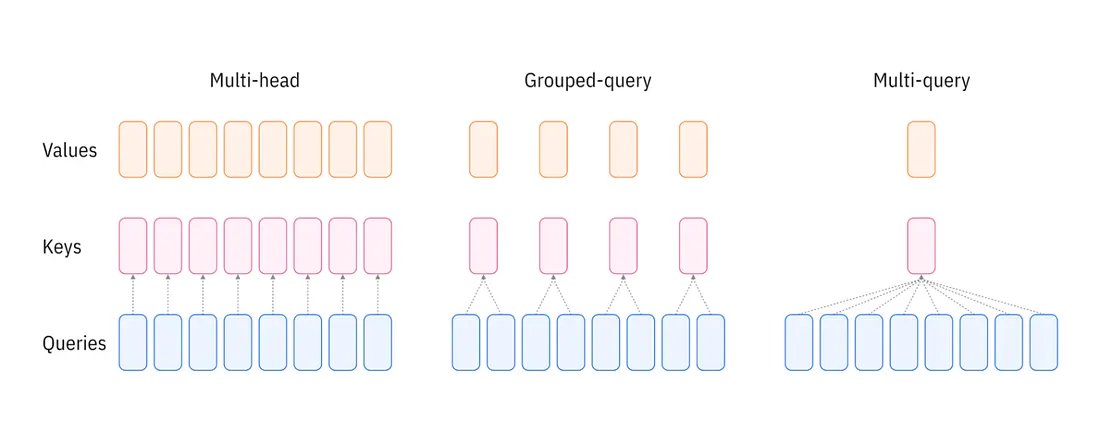
\includegraphics[width=0.55\textwidth]{GQA.png}
	\caption{An structural overview of the Grouped-Query Attention (GQA) mechanism compared alongside Multi-Head Attention (MHA) and Multi-Query Attention (MQA)~\cite{ainslie2023gqa}.}\label{fig:GQA}
\end{figure*}

Ainslie et al.~\cite{ainslie2023gqa} introduces Grouped-Query Attention (GQA), which groups multiple query heads to share same key and value, as shown in Fig.~\ref{fig:GQA} reducing cache size while losing little output quality. GQA stays in between two attention techniques: standard Multi-Head Attention (MHA), where each query head has its own key and value,and Multi-Query Attention (MQA), where all query heads share a single key and value.

The result from the experiment shows that GQA inference speed is close to that of Multi-Query Attention (MQA) and maintains performance similar to that of standard Multi-Head Attention. The authors also introduce an effective way to upgrade existing MHA models into GQA models using mean pooling, requiring only a small amount of time and cost to adapt~\cite{ainslie2023gqa}.

\subsection{KV Cache Quantization}
KV Cache Quantization is the optimization technique which is used to reduce memory requirement to store key and value tensors. Normally, these tensors are stored in high precision format usually FP16, instead of that these cached tensors are represented in lower precision format such as FP8, FP4. This helps in decreasing memory footprint and allows longer context length while maintaining model accuracy~\cite{nvidia2025nvfp4}.

To reduce memory usage, multiple studies have introduced different KV cache quantization methods. FP8 KV cache is widely used because of its balance in memory savings and in model accuracy. A newer method, NVFP4 KV cache has been introduced by NVIDIA, which stores key and value tensors in 4-bit floating point format, reducing KV cache memory by half compared to that of FP8, allowing longer context lengths, supports more users, and lowers memory bandwidth during decoding. Cached values are dequantized for attention computation and quantized again before being stored~\cite{nvidia2025nvfp4}.

Another method is MixQuant~\cite{lu2026mixquant} which uses mixed precision quantization by providing different precision levels to different cached tensors based on their importance. This reduce memory while maintaining better accuracy than using low level precision for all tensors.

MiniKV~\cite{sharma2025minikv} improves efficiency of KV cache by combining 2-bit quantization and removes less important cached tokens. It not only reduce size of KV cache through quantization, it also frees memory by keeping only the most useful information. MiniKV reduces KV cache memory by more than 80\% while maintaining accuracy and providing faster inference than methods that use only quantization.
\begin{table}[htbp]
	\centering
	\caption{Comparison of KV cache quantization techniques.}
	\label{tab:kv_quantization}
	\small
	\begin{tabularx}{\linewidth}{llXX}
		\toprule
		\textbf{Method} & \textbf{Precision}        & \textbf{Main Benefit}            & \textbf{Trade-off}    \\
		\midrule
		FP16            & 16-bit                    & Highest accuracy                 & Large memory usage    \\
		\midrule
		FP8             & 8-bit                     & Lower memory                     & Slight accuracy loss  \\
		\midrule
		NVFP4           & 4-bit                     & Smaller cache                    & Quantization overhead \\
		\midrule
		MixQuant        & Mixed precision           & Better accuracy-memory trade-off & Higher complexity     \\
		\midrule
		MiniKV          & 2-bit + adaptive eviction & 80\% compression                 & Custom kernels        \\
		\bottomrule
	\end{tabularx}
\end{table}

Table~\ref{tab:kv_quantization} summarizes recent KV cache quantization techniques based on the findings in~\cite{nvidia2025nvfp4,lu2026mixquant,sharma2025minikv}.

Although KV Cache Quantization reduces memory usage, it reduces generation quality for a longer context because of using low precision tensor format. As a result, current research focuses on finding the right balance between memory efficiency and model accuracy to enable the practical deployment of modern LLMs~\cite{nvidia2025nvfp4,lu2026mixquant,sharma2025minikv}.

\subsection{KV Cache Compression}
When context length increases, the KV cache occupies a large portion of GPU memory. While quantization reduces the precision of cached tensors, KV-cache compression decreases the amount of information stored within the key-value representations by removing redundancy. It reduces memory consumption while preserving the necessary information for accurate results~\cite{shan2025cognitivememoryllms}.

Many studies have provided different ways to reduce the size of KV cache. One way is low-rank compression, which stores the key and value information in a smaller form while keeping most important informations. Another method is KV merging, where similar key value pairs are combined which reduce the number of stored entries. Recent studies use multi-level compression by keeping important tokens in better quality while compressing less important or older tokens to save memory~\cite{shan2025cognitivememoryllms}.

Chang et al.~\cite{chang2025xkv} found that KV caches from nearby transformer layers contain similar information. Instead of storing the KV cache for every layer separately, xKV uses Singular Value Decomposition (SVD) to combine similar information from multiple layers into a smaller shared representation. This helps reduce the amount of memory needed while still maintaining good model accuracy. xKV can reduce the KV cache size by up to 8$\times$, and when it is combined with 4-bit quantization, the compression increases to 25.6$\times$ with only a small reduction in accuracy.

This shows that xKV can be used together with other methods, such as quantization and intra-layer compression. Rather than replacing these techniques, xKV helps improve memory savings when they are used together.

\begin{table}[htbp]
	\centering
	\caption{Overview of KV Cache Compression Techniques~\cite{shan2025cognitivememoryllms,chang2025xkv}.}
	\label{tab:kv_compression}
	\small
	\begin{tabularx}{\linewidth}{lXXX}
		\toprule
		\textbf{Technique} & \textbf{Principle}                                               & \textbf{Advantage}            & \textbf{Limitation}         \\
		\midrule
		Low-Rank           & Project KV tensors into lower-dimensional space                  & Lower memory usage            & Reconstruction error        \\
		\midrule
		KV Merging         & Merge similar KV pairs                                           & Smaller cache size            & Possible information loss   \\
		\midrule
		Multi-Level        & Apply different compression levels                               & Better memory-quality balance & More complex implementation \\
		\midrule
		Cross-Layer (xKV)  & Share a low-rank representation across multiple layers using SVD & Up to $8\times$ compression   & Extra SVD computation       \\
		\bottomrule
	\end{tabularx}
\end{table}


Although KV cache compression uses less GPU memory and allow the model to handle longer input without using too much extra memory, compare to that of normal KV cache. If the data is compressed too much, some important information may be lost, which can reduce the quality of the output.

\subsection{Memory Management}
\label{sec:memory}
When input becomes longer, the KV cache also becomes larger, which increases memory usage. Memory management techniques helps to store, organize, and access the KV cache more efficiently during inference. Unlike quantization and compression, memory management does not reduce the KV cache size. Instead, it uses hardware memory more efficiently allowing longer inputs.

Offloading moves less frequently used parts of KV cache from GPU memory to other storage. When that data is needed, it is moved back to the GPU. This reduces GPU memory usage and allows longer context lengths, but moving data between different storage levels can increase latency~\cite{sheng2023flexgen}.

PagedAttention uses similar method as virtual memory in operating systems by dividing the KV cache into small fixed-size pages. Instead of assigning a large memory space for each request, it only uses memory pages. This reduces memory waste, and allows more requests to run together~\cite{kwon2023vllm}.

Shared Attention reduce memory usage by allowing different requests to share the same KV cache when they have similar prompts. It avoids storing the same information again and reduces extra computation, which improve performance when many users are using the model~\cite{fawaz2024beyond}.
\begin{table}[htbp]
	\centering
	\caption{Comparison of KV cache memory management techniques.}
	\label{tab:kv_management}
	\small
	\begin{tabularx}{\linewidth}{lXXX}
		\toprule
		\textbf{Technique} & \textbf{Main Idea}       & \textbf{Advantage}     & \textbf{Limitation}            \\
		\midrule
		Offloading         & Move KV cache to CPU     & Lower GPU memory usage & Transfer latency               \\
		\midrule
		PagedAttention     & Page-based KV allocation & Better GPU utilization & More complex memory management \\
		\midrule
		Shared Attention   & Reuse common KV cache    & Higher throughput      & Requires shared contexts       \\
		\bottomrule
	\end{tabularx}
\end{table}


\subsection{Synthesis: A Comparative Decision Framework}
\label{sec:synthesis}
Sections~\ref{sec:attention} to~\ref{sec:memory} reviewed four different categories KV cache optimization techniques:attention-level redesign, quantization, compression, and memory management. Although each category aim to solve same problem of the linear growth of KV cache size with context length described in Equation~\eqref{eqn:KVcachesize}, each method focuses on a different part of the inference process and solves different performance issues. Table~\ref{tab:synthesis} provides a summary of these techniques and compares them based on the main bottleneck they address

\begin{table*}[htbp]
	\centering
	\caption{Comparative synthesis of KV cache optimization techniques across all categories.}
	\label{tab:synthesis}
	\small
	\begin{tabularx}{\linewidth}{llXXXX}
		\toprule
		\textbf{Technique} & \textbf{Category}         & \textbf{Primary Bottleneck Addressed}    & \textbf{Memory/Latency Impact}                                & \textbf{Accuracy Trade-off}       & \textbf{Best-Fit Scenario}                               \\
		\midrule
		GQA                & Attention-Level           & Redundant computation across query heads & Reduces cache size at the architectural level; near-MQA speed & Minimal loss                      & General-purpose, latency-sensitive single-user inference \\
		\midrule
		FP8                & Quantization              & GPU memory capacity                      & $\sim$50\% memory reduction vs.\ FP16                         & Slight loss                       & Balanced, general-purpose deployment                     \\
		NVFP4              & Quantization              & Memory capacity and bandwidth            & Halves FP8 cache size, lowers bandwidth                       & Moderate loss                     & Very long context, many concurrent users                 \\
		MixQuant           & Quantization              & Memory-accuracy balance                  & Variable, tensor-dependent                                    & Better than uniform low precision & Accuracy-sensitive tasks needing memory savings          \\
		MiniKV             & Quantization + Eviction   & Memory capacity                          & $>$80\% compression, hardware co-design improves throughput   & Retained via adaptive eviction    & Long-context serving under strict memory limits          \\
		\midrule
		Low-Rank           & Compression               & Memory capacity                          & Moderate reduction                                            & Reconstruction error              & Memory-constrained, accuracy-tolerant settings           \\
		KV Merging         & Compression               & Memory capacity                          & Moderate reduction                                            & Possible information loss         & Moderate compression needs                               \\
		Multi-Level        & Compression               & Memory-quality balance                   & Adaptive, token-importance-driven                             & Balanced                          & Long documents with varying token importance             \\
		xKV                & Compression (cross-layer) & Memory capacity                          & Up to 8$\times$, 25.6$\times$ combined with quantization      & Minimal loss                      & Very long context; stacks with quantization              \\
		\midrule
		Offloading         & Memory Management         & GPU memory capacity                      & Lower GPU usage; adds transfer latency                        & Lossless                          & Memory-constrained GPUs, latency-tolerant                \\
		PagedAttention     & Memory Management         & Memory fragmentation/utilization         & Better GPU utilization, higher throughput                     & Lossless                          & Multi-tenant serving systems                             \\
		Shared Attention   & Memory Management         & Redundant computation across users       & Higher throughput for similar prompts                         & Lossless                          & High-concurrency, shared-prompt workloads                \\
		\bottomrule
	\end{tabularx}
\end{table*}

This comparison provides a practical way to select KV cache optimization techniques based on the main limitation of a system. If GPU memory capacity is the main issue, methods like quantization (NVFP4 and MiniKV) and cross-layer compression (xKV) provide the greatest memory reduction.

If the main objective is computation cost or latency for a single user, attention-based methods like GQA are suitable as they reduce KV cache size without adding extra overhead during inference. For systems that supports many users at the same time, memory management techniques such as Paged Attention and Shared Attention are effective because they improve GPU memory usage and increase throughput without changing the cache precision.

If model accuracy is the main priority, techniques such as MixQuant and multi-level compression provide a better balance between memory reduction and accuracy compared to applying low precision. Overall, these methods are not alternatives where only one can be used. They can work together, and combining techniques like quantization and memory management can help achieve better performance when deploying large LLMs.

\section{Methodology}
\subsection{Theoretical Framework and Justification}

In existing research, different KV cache optimization methods are discussed seperately, and different studies use different ways to categories these techniques. To provide a consistent comparison, this report organizes KV cache optimization methods using a \textit{bottleneck-oriented taxonomy}. Each technique is categorized based on the part of the KV cache system it improves. Some methods reduce factors in the KV cache size equation (Eq.~\eqref{eqn:KVpertoken}), while others focus on improving cache storage and access.

Equation~\eqref{eqn:KVpertoken} shows that the KV cache size depends on four main factors: the number of attention heads ($H$), the number of transformer layers ($L$), the bytes used for each element ($B$), and the head dimension ($D$). Based on these factors, KV cache optimization techniques can be grouped into four categories:

\begin{itemize}
	\item \textbf{Attention-level techniques} (e.g., GQA) reduce the effective number of attention heads ($H$) by allowing multiple query heads to share key-value projections.

	\item \textbf{Quantization techniques} (e.g., FP8, NVFP4, MiniKV) reduce the bytes per element ($B$) by using lower numerical precision.

	\item \textbf{Compression techniques} (e.g., low-rank compression, xKV) reduce redundant information stored in the KV cache by compressing representations across layers or within the cache.

	\item \textbf{Memory management techniques} (e.g., PagedAttention and offloading) do not reduce the actual KV cache size. Instead, they improve how the cache is stored, managed, and accessed during inference.
\end{itemize}

Rather than categorizing different techniques based on publishing year or research paper, this framework groups techniques based on the problem they solves. This makes it easier to compare different methods and understand which technique is more suitable for different situations.

\subsection{Research Design}

This study follows a \textit{comparative literature survey design} based on the bottleneck-oriented taxonomy introduced in the previous subsection. Instead of collecting new experimental results, it reviewed and compares findings from existing research papers. Since one single paper introduces many different techniques and same techniques may be discussed in multiple different sources, rather than focusing on research papers, it focuses on analysis of each KV cache optimization technique.

Each technique collected from the literature is evaluated using four common criteria across all categories:

\begin{itemize}
	\item \textbf{Memory impact} is measured by how much the technique reduces KV cache size or GPU memory usage.
	\item \textbf{Latency/throughput impact} describes how the technique affects inference speed, response time, and serving performance.
	\item \textbf{Accuracy trade-off} considers whether the technique causes any reduction in model performance or output quality.
	\item \textbf{Implementation complexity} evaluates the difficulty of applying the technique, including the need for model changes, retraining, or specialized hardware support.
\end{itemize}

Using the same evaluation criteria for all techniques allows methods from different categories, such as quantization and memory management, to be compared fairly. This consistent comparison approach supports the cross-category analysis and decision framework presented in Section~\ref{sec:synthesis}, where techniques are evaluated based on their advantages, limitations, and suitable application scenarios.

\subsection{Complexity Analysis Procedure}
\label{sec:complexity}

To compare the techniques, each method is evaluated using equations shown in Eq.~\eqref{eqn:KVpertoken} and~\eqref{eqn:KVcachesize}. If a paper already provides experimental results, such as compression ratios or memory savings, those results are used directly. If it doesn't we just replace variable in the formulas based on the changes (e.g. head grouping, low-rank compression, token pruning), made in each technique. Simlarly for quantization techniques (like INT8 or FP4 quantization) which uses lower precision, evaluation is done by shrinking the bytes per number without changing how the math or complexity works.

Discussion of computational complexity and memory complexity is done seperately. Although KV caching avoids recomputing the Key and Value for tokens that have already been generated, each new token still needs to attend to all previously cached tokens. Therefore, decoding complexity does not change. Instead, most KV cache optimization techniques improve inference performance by reducing memory usage, memory bandwidth, or runtime overhead.

\textbf{Baseline.} Without a KV cache, autoregressive decoding recomputes the Key and Value projections for all previously generated tokens at every decoding step. When generating $i$-th token, it has to process all previous $i-1$ tokens again. As this process is repeated for every new token, the total computational complexity becomes

\[
	\sum_{i=1}^{N}O(i)=O(N^2).
\]

The KV cache stores the previously computed Key and Value vectors, so they do not need to be recomputed during decoding. When a new token is generated, only its Key and Value vectors are calculated, while attention is still performed over all previously cached tokens. Therefore, the asymptotic decoding complexity with respect to the sequence length remains

\[
	O(N^2),
\]

Although the asymptotic complexity remains the same, the actual computational cost is much lower, resulting in faster inference and higher throughput~\cite{xu2026kv}.

Based on Eq.~\eqref{eqn:KVpertoken} and~\eqref{eqn:KVcachesize}, the KV cache memory requirement can be expressed as:

\[
	O(L \cdot H \cdot D \cdot B \cdot N).
\]

%GQA

\textbf{Attention-Level (GQA).} In standard Multi-Head Attention (MHA), each query head has its own Key-Value (KV) head, which is why the memory requirement includes the factor $H$ in Eq.~\eqref{eqn:KVpertoken}. Grouped Query Attention (GQA) reduces memory usage by allowing multiple query heads to share the same Key-Value (KV) head. Instead of having $H$ query heads, query head are divided into $g$ groups that share a single Key-Value head, reducing the number of stored KV heads from $H$ to $H/g$~\cite{ainslie2023gqa}. Therefore, by replacing  $H$ with $H/g$ the memory complexity becomes

\[
	O\left(
	L\cdot\frac{H}{g}\cdot D\cdot B\cdot N
	\right).
\]

This reduces the KV cache memory usage and the amount of memory bandwidth needed during inference, while keeping the same overall decoding complexity.

%Quantization

\textbf{Quantization (FP8/NVFP4/MiniKV).} Quantization reduces the number of bytes used to store each element, which decreases value of $B$ in Eq.~\eqref{eqn:KVpertoken}. Other factors $L$, $H$, $D$, or $N$ are not modified. For example, FP8 uses half the storage of FP16, while NVFP4 uses half the storage of FP8~\cite{nvidia2025nvfp4}. Replacing  $B$ with smaller $B'$ gives

\[
	O(L\cdot H\cdot D\cdot B'\cdot N).
\]

Since $B'$ is only a smaller constant than $B$, quantization does not change the overall asymptotic memory complexity. Instead, it reduces the amount of memory required by a constant factor. MiniKV further improves memory efficiency by combining low-precision storage with adaptive token selection. Instead of keeping all $N$ tokens in the KV cache, it only selects $N'$ important tokens, where $N'< N$. As a result, the memory complexity is reduced to

\[
	O(L\cdot H\cdot D\cdot B'\cdot N'),
\]

Experimental results show that MiniKV can reduce KV cache memory by more than 80\%~\cite{sharma2025minikv}.

%Compression

\textbf{Compression (Low-Rank / xKV).} Low-rank compression reduces the size of the head dimension by representing it with a lower-dimensional rank $r$, where $r<D$. This decreases the amount of memory needed to store the KV cache. Replacing $D$ with $r$ in the memory equation gives

\[
	O(L\cdot H\cdot r\cdot B\cdot N)
\]

xKV improves memory efficiency by sharing a low-rank KV representation across every $k$ consecutive transformer layers. This shared representation is obtained using Singular Value Decomposition (SVD)~\cite{chang2025xkv}. By sharing the KV representation across multiple layers, the effective number of stored layer representations is reduced from $L$ to $L/k$. Therefore, the memory complexity becomes

\[
	O\left(
	\frac{L}{k}\cdot H\cdot D\cdot B\cdot N
	\right),
\]

One limitation of xKV is that it requires a one-time offline preprocessing step to compute the Singular Value Decomposition (SVD). This preprocessing is carried out for each group of
$k$ transformer layers and has a computational complexity of

\[
	O(D^2\cdot k)
\]

%Memory Management

\textbf{Memory Management (PagedAttention).} Memory management techniques do not change the KV cache memory complexity shown in Eq.~\eqref{eqn:KVpertoken}. Therefore, the overall memory requirement remains

\[
	O(L\cdot H\cdot D\cdot B\cdot N).
\]

Instead of reducing the size of the KV cache itself, these techniques improves memory allocation and utilization. In traditional contiguous memory allocation memory is reserved based on maximum possible length which leads to internal fragmentation (unused memory). PagedAttention solves this issue by dividing KV cache into fixed sized pages and memory is allcoated only when needed~\cite{kwon2023vllm}. Therefore, memory waste is bounded by

\[
	O(\text{page size})
\]

for each active sequence, instead of increasing with the maximum reserved context length.

%runtime

\bibliographystyle{IEEEtran}
\bibliography{reference}

\end{document}